\documentclass[a4paper]{article}

\usepackage{INTERSPEECH2019}
\usepackage{hyperref}
\usepackage{comment}
\usepackage{multirow}
\title{Status Report 2: Mar. $8^{th}$}
\name{Liming Wang$^1$}
\address{University of Illinois, Urbana Champaign}
\email{lwang114@illinois.edu}

\begin{document}
\maketitle
\section{Model Description}
% Normalize over concepts vs. normalize over time
\begin{figure}
    \centering
    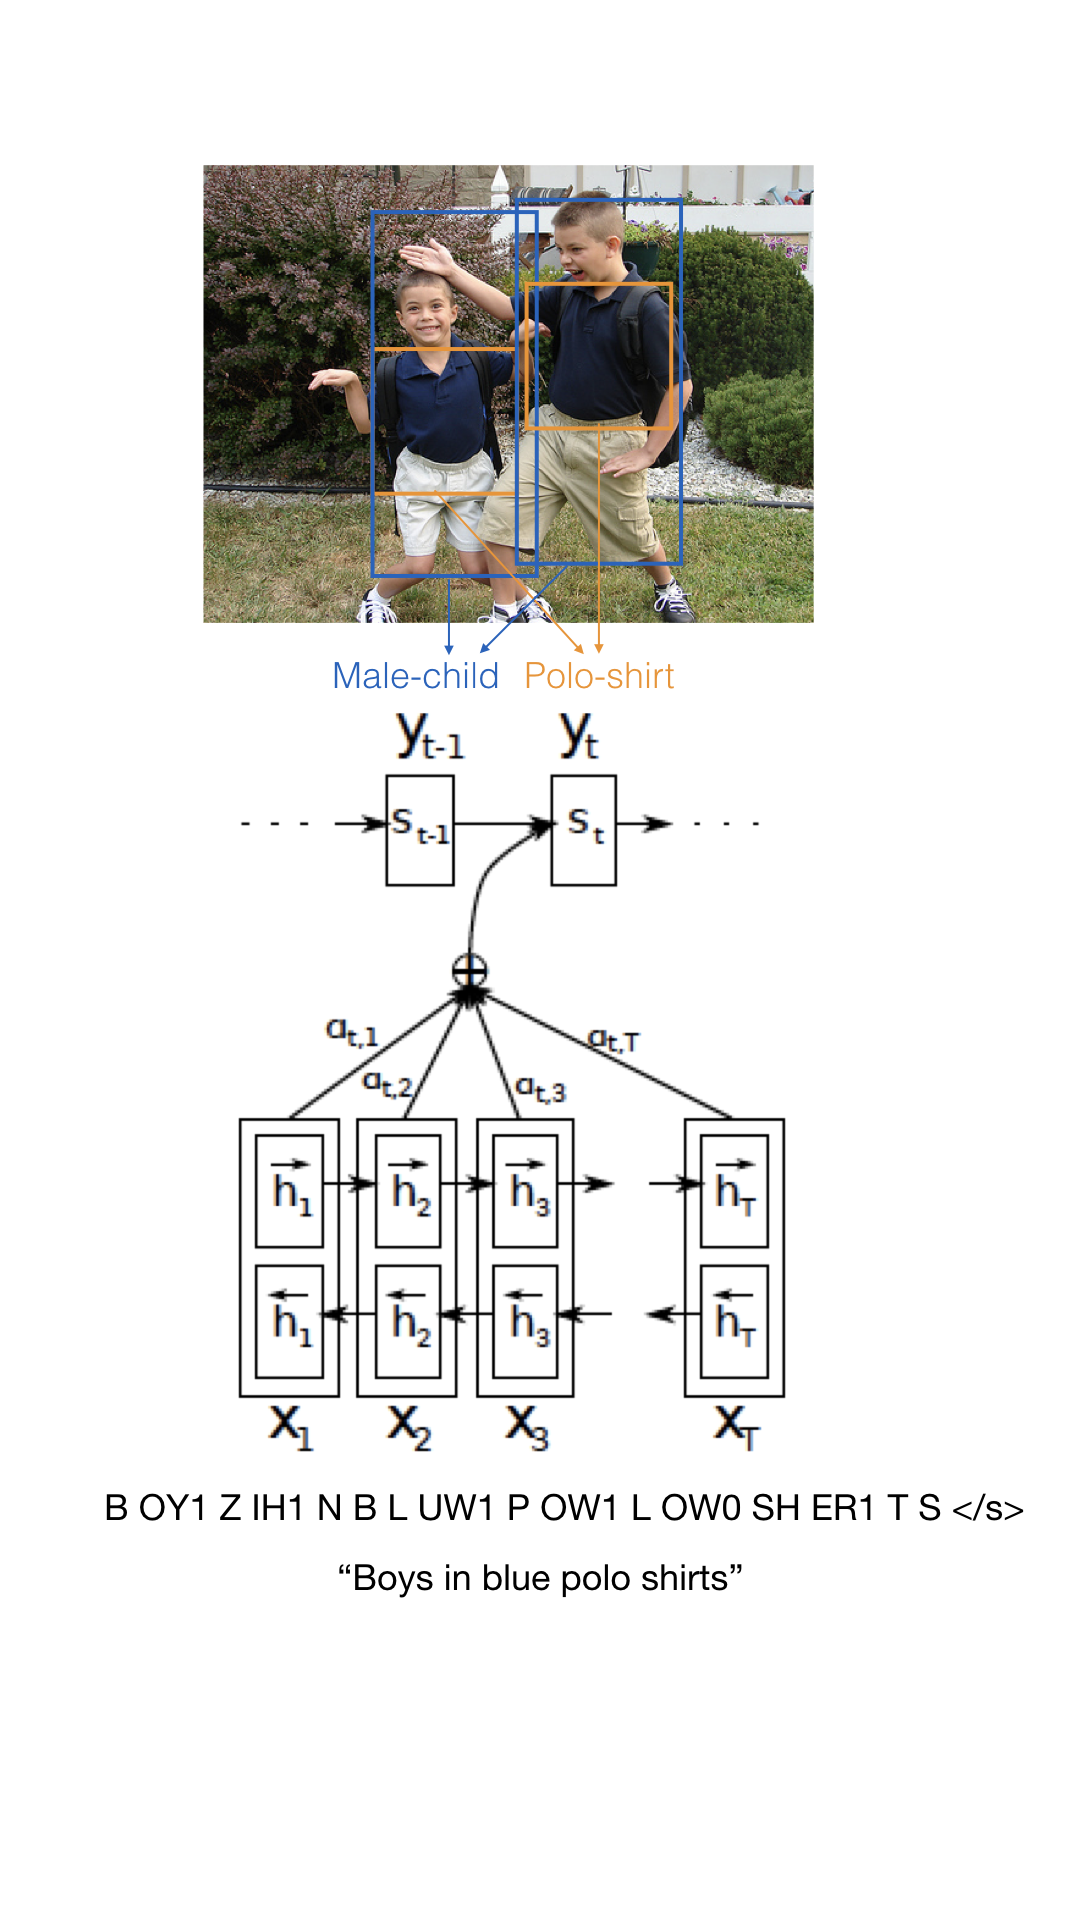
\includegraphics[width=0.4\textwidth]{status_report2_mar8th/nmt_model.png}
    \caption{Caption}
    \label{fig:my_label}
\end{figure}
\begin{figure}
    \centering
    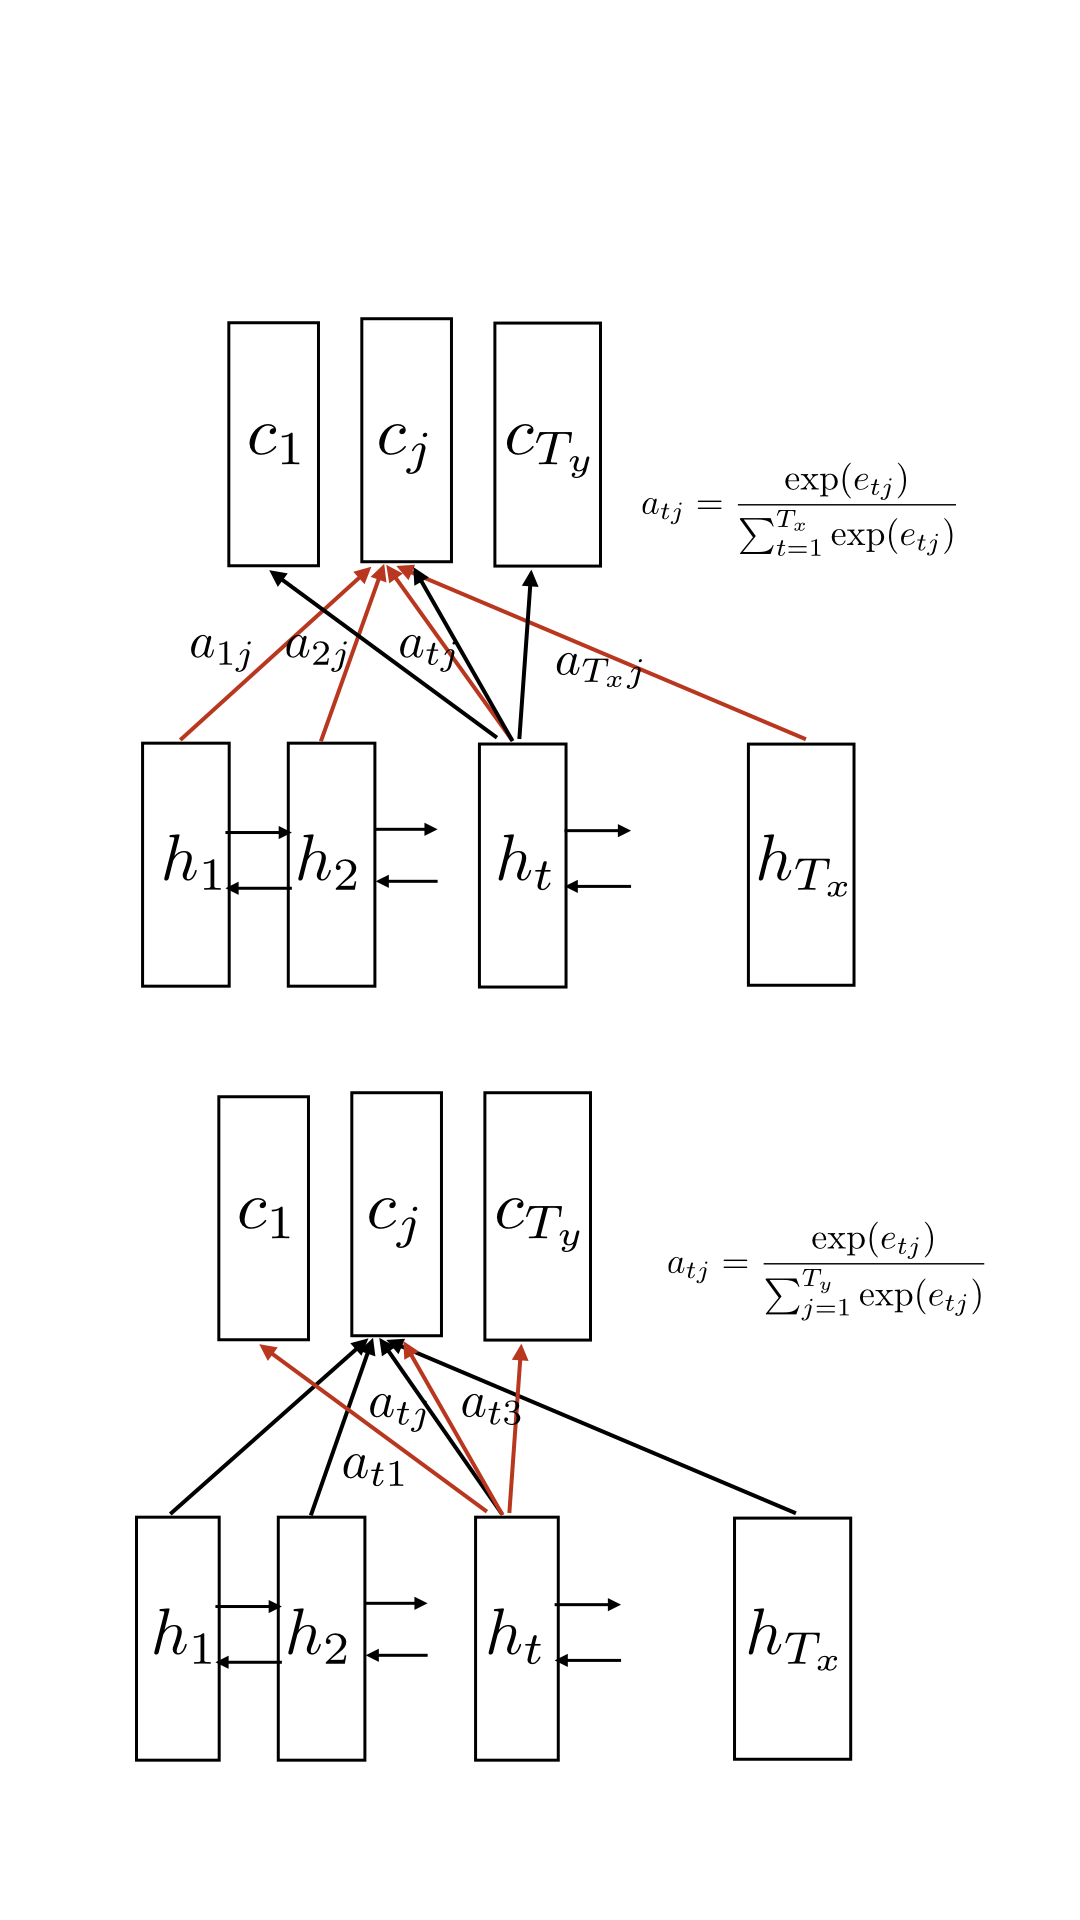
\includegraphics[width=0.2\textwidth]{status_report2_mar8th/norm_ov_time_vs_concept.png}
    \caption{Caption}
    \label{fig:my_label}
\end{figure}
\begin{figure}
    \centering
    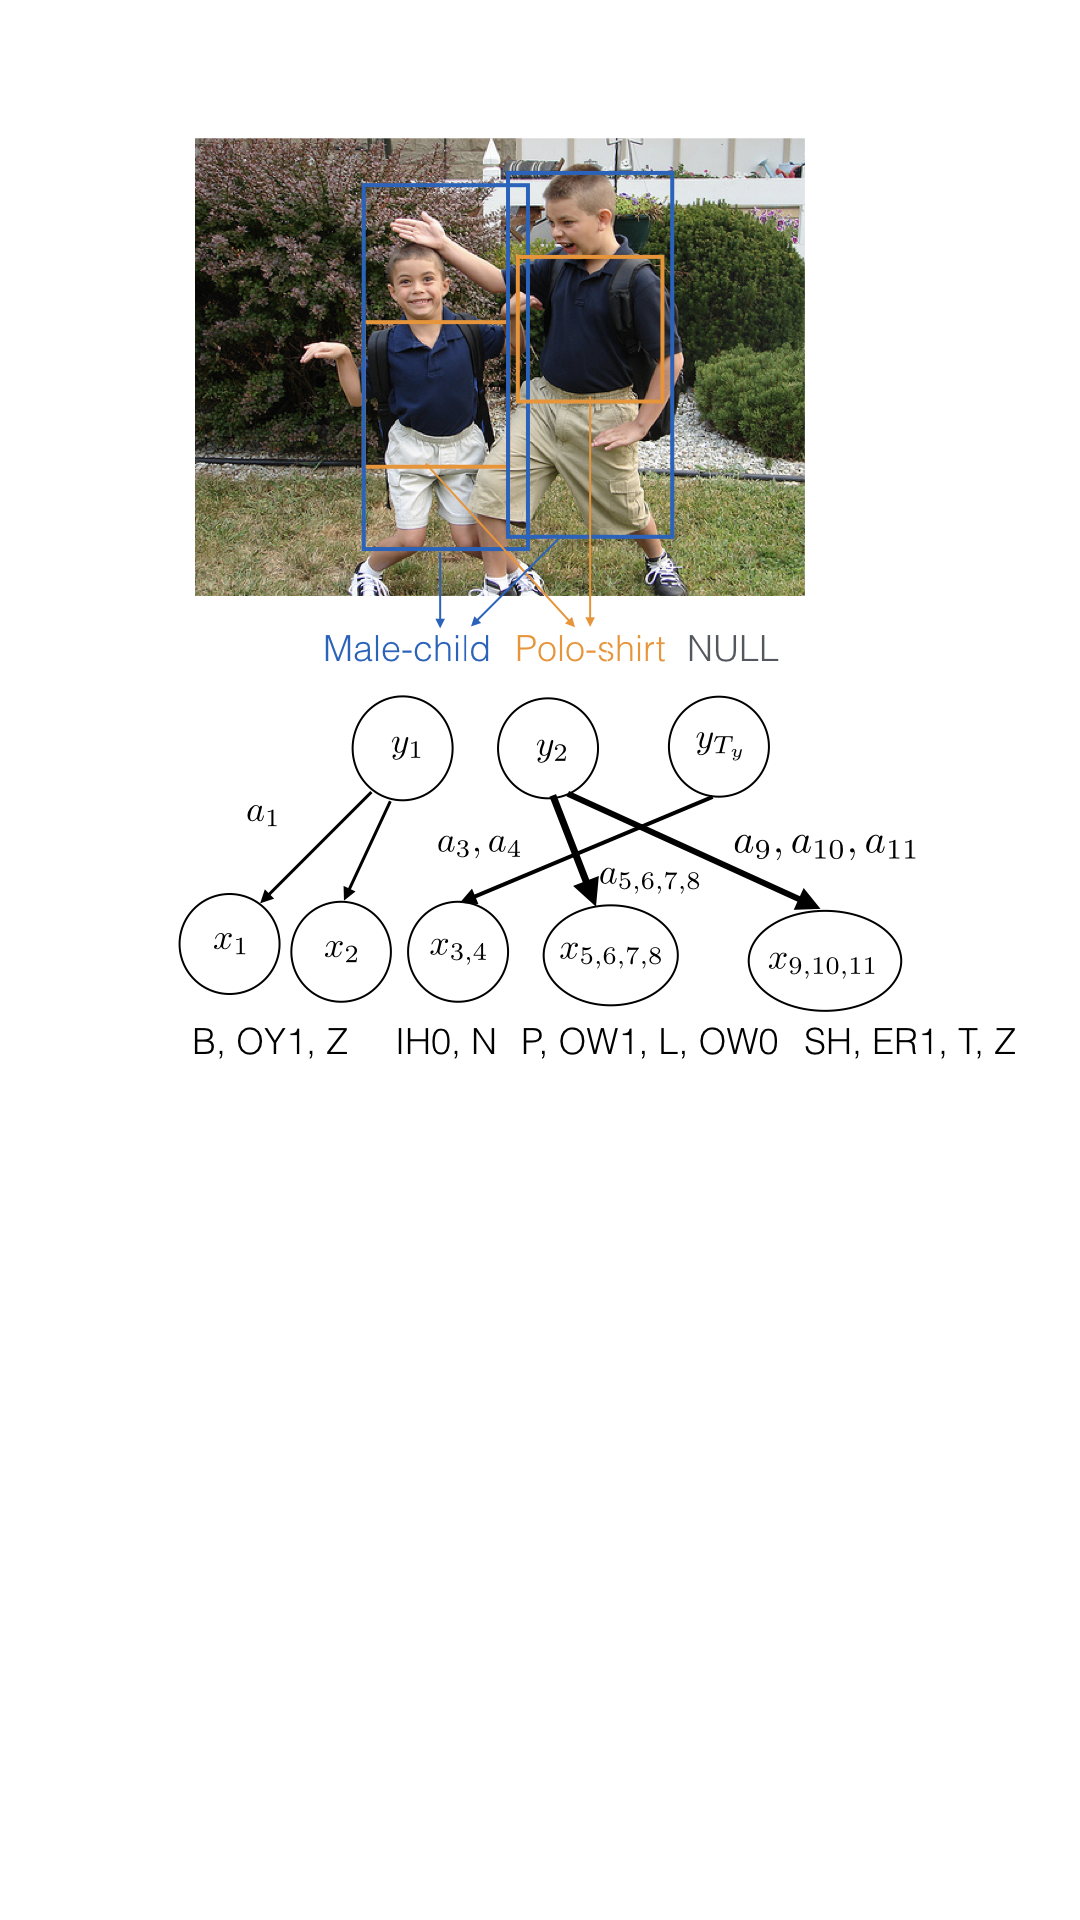
\includegraphics[width=0.2\textwidth]{status_report2_mar8th/smt_model.png}
    \caption{Caption}
    \label{fig:my_label}
\end{figure}

% SMT vs. NMT

\section{Experiments}
\subsection{Dataset}
% Dataset description
We use the Flickr30kEntities dataset to extract the image concepts and phoneme sequences. Only the images appeared in Flickr8k is used for comparison with other speech-to-image models like \cite{Harwath16-ULO}. Also we restricted our attention to a list of concepts that appeared at least 10 times in the Flickr8k dataset and created a set of 1547 image concepts using Wordnet synsets (cite needed). The captions are converted into phoneme sequences via the CMU pronunciation dictionary (cite needed) which contains 39 distinct phonetic symbols and 69 symbols in total with the stress symbol. Compound words such as ``fingerpaint'' or ``skateboarder'' do not have an entry in the dictionary, and we simply replace them with an \textt{UNK} symbol. Each caption corresponds to only one image and each image has five captions.

% Dataset conception distribution
The frequency distribution of image concepts and number of objects per caption is shown below. 

\subsection{Word Discovery Results}
% Setup
\begin{align*}
    \mathbf{Rec}_i^{(s)} &= \frac{\sum_{j=1}^{T_x^{(s)}} \mathbf 1 [a_j^{(s)} = \hat{a}_j^{(s)} = i]}{\sum_{j=1}^{T_x^{(s)}} \mathbf 1 [a_j^{(s)} = i]}\\
    \mathbf{Prec}_i^{(s)} &= 
     \frac{\sum_{j=1}^{T_x^{(s)}} \mathbf 1 [a_j^{(s)} = \hat{a}_j^{(s)} = i]}{\sum_{j=1}^{T_x^{(s)}} \mathbf 1 [\hat{a}_j^{(s)} = i]}.
\end{align*}
The final recall and precision scores are then:
\begin{align*}
    \mathbf{Recall} &=  \frac{1}{N}\sum_{s=1}^{N}
    \frac{\sum_{i=1}^{T_y}\mathbf{Rec}_i^{(s)}}{T_y}\\
    \mathbf{Precision} &= \frac{1}{N}\sum_{s=1}^{N} \frac{\sum_{i=1}^{T_y}\mathbf{Prec}_i^{(s)}}{T_y}\\
    \mathbf{F-measure}(a(x), \hat{a}(x)) &= \frac{2}{\mathbf{Recall}^{-1}+\mathbf{Precision}^{-1}}
\end{align*}


We trained both our statitical and neural word discoverers on phoneme-concept pairs from Flickr30k. For the statistical model, we extracted the Viterbi alignment for each pair; for the neural model, we extracted the attention weights of the model and generated the optimal alignment by taking the image concepts associated with the maximal weight for a given phoneme. In both cases, the pseudo-word unit is then the sequence of consecutive phonemes that align to the same image concept. For comparison, we also report the word discovery results obtained by the standard neural machine translation model with attention weights normalized over the input phoneme sequence. 

% Attention weights for the two nmt model

% Evolution of atttention weights over training epochs

% Prob distribution examples for a given word in the SMT + evolution across training epochs
\begin{table}[ht]
    \centering
    \caption{Phoneme Probability distribution for the word ``cat'' learnt by the SMT model}
    \begin{tabular}{|c|c|}
        \hline
        & $P[\pi|l=\text{cat}]$\\
        \hline
        K & 0.165\\
        AE1 & 0.116\\
        T & 0.161 \\
        *AH0 & 0.063\\
        *N & 0.059 \\
        *B & 0.049 \\
        *L & 0.044 \\
        *D & 0.039 \\
        *EH1 & 0.028\\
        \hline
    \end{tabular}
    \label{tab:my_label}
\end{table}

% Alignment length (nmt vs smt)

% # of aligned objects (nmt vs smt)

% accuracy, wordIoU, ROC curve
\begin{table}[th]
    \centering
    \caption{SMT vs NMT: Word Discovery Results}
    \begin{tabular}{|c|c|c|c|}
    \hline
        & \multirow{2}{*}{SMT} & NMT  & NMT\\
        & & (norm. over concepts) & (norm. over time)\\
    \hline
    Word-IoU & 6. & 46.0 & 35.6 \\
    Accuracy & 43.8 & 23.0 & 18.5 \\
    Recall   & 52.9 & 18.0 & 26.8 \\
    Precision & 46.7 & 12.1 & 5.58 \\
    F-Measure & 49.6 & 14.5 & 9.24\\
    \hline
    \end{tabular}
    \label{tab:word_discovery_res}
\end{table}

\subsection{Retrieval Results}
We applied our word discoverer to the task of image retrieval. We split the flickr30k dataset into training and test set, with the test set being the same as described in \cite{Karpathy16-CIA}. For each image example we compute the translation probability of the phoneme sequence given the image concepts: $P[x_1\ldots x_{T_x}|y_1\ldots y_{T_y}]$. For phoneme-translation pair unseen before, we simply filled in for the pair a small fixed probability $10^{-12}$. 
% Retrieval accuracy with comparison to HG 15
\begin{table}[th]
    \centering
    \caption{SMT vs NMT: Phoneme-to-image Retrieval Results}
    \begin{tabular}{|c|c|c|c|}
    \hline
             & Recall@1 & Recall@5 & Recall@10\\
             \hline
         SMT & 20\% & 47\% & 55\% \\
         NMT (norm. over concepts) &  &  &  \\
         Harwath\&Glass & - & - & 17.9\% \\
         Karpathy \cite{Karpathy16-CIA} &- &- & 42.5\%\\
         \hline
    \end{tabular}
    \label{tab:retrieval_res}
\end{table}

\subsection{Error Analysis}
One source of error may be that the image concept is noisy. The wordnet synset does not contain entries for compound nouns such as ``entry way'', which was classified incorrectly as ``manner'' because only ``way'' is taken into account. 

% Alignment confused by rare words

% Context dependency

% Confusion between similar-sounding words

% Concepts not annotated in the image

% Retrieval confusion

% Overfitting
For the attention-based model, due to a scarsity of data, the network tends to ignore the less frequent image concepts and put all the weights on the more common concepts; the problem is more serious for the attention normalized over time, when in many instances the attention weights are constant through all the concepts.

\end{document}